\documentclass[
	% -- opções da classe memoir --
	12pt,				% tamanho da fonte
	openright,			% capítulos começam em pág ímpar (insere página vazia caso preciso)
	oneside,			% para impressão em um lado. Oposto a twoside, verso e anverso
	a4paper,			% tamanho do papel. 
	% -- opções da classe abntex2 --
	chapter=TITLE,		% títulos de capítulos convertidos em letras maiúsculas
	section=TITLE,		% títulos de seções convertidos em letras maiúsculas
	%subsection=TITLE,	% títulos de subseções convertidos em letras maiúsculas
	%subsubsection=TITLE,% títulos de subsubseções convertidos em letras maiúsculas
	% -- opções do pacote babel --
	english,			% idioma adicional para hifenização
	%french,				% idioma adicional para hifenização
	spanish,			% idioma adicional para hifenização
	brazil,				% o último idioma é o principal do documento
	]{styles/abntex2}

\usepackage{titlesec}
\usepackage[alf,abnt-etal-list=0,abnt-etal-cite=3,abnt-repeated-author-omit=no,abnt-doi=expand,abnt-emphasize=bf]{styles/abntex2cite}	% Citações padrão ABNT
\usepackage[utf8]{inputenc}
\usepackage[T1]{fontenc}
\makeatletter
\usepackage[singlelinecheck=false,justification=raggedright]{caption}
\usepackage{lastpage}
\usepackage{tabularx}
\usepackage{times}
\usepackage{graphicx}
\usepackage{styles/ttc_univali}
\usepackage{lipsum}
\usepackage{url}
\usepackage[table,xcdraw]{xcolor}
\usepackage{float}
\usepackage{accents}
\usepackage{array}
\usepackage{hyphenat}
\usepackage{multirow}
\newcolumntype{C}[1]{>{\centering\arraybackslash}m{#1}}

%\newcolumntype{C}[1]{>{\centering\let\newline\\\arraybackslash\hspace{0pt}}m{#1}
% \usepackage[
%     % showframe=true
%     ]
% {geometry}

\title{TTC Engenharia da Computação}
\author{Modelo from Stephen Michael Apolinário}
\date{August 2022}

\hyphenation{op-tical net-works customiza-cao implementa-cao quan-do microcon-troladores} 

\begin{document}
\titleformat*{\subsubsection}{\normalfont}
\renewcommand{\arraystretch}{1.10}
\pretextual

\begin{Info}
    % Universidade
    {UNIVERSIDADE DO VALE DO ITAJAÍ}
    % Escola
    {ESCOLA DO MAR, CIÊNCIA E TECNOLOGIA}
    % Curso
    {CURSO DE ENGENHARIA DE COMPUTAÇÃO}
    % Titulo
    {relatório 03}
    % Autor
    {Stephen Michael Apolinário}
    % Cidade e Data
    {Itajaí (SC), agosto de 2022}
    % Nome da Área de concentração
    {Modelos de análise do diodo}
    % Orientador(a)
    {Walter Gontijo}
    % Coorientador(a) <Nome do Coorientador(a)>, <Titulação> %%%%%%%% Se não tiver coorientador deixe vazio
    {}
    \end{Info}
    
    % \begin{Dedicatoria}
    % Este elemento é opcional, mas caso queira fazer uma dedicatória, preencha aqui.
    % \end{Dedicatoria}
    
    % \begin{Agradecimentos}
    % Os agradecimentos são opcionais, mas este é o local adequado para isso.
    % \end{Agradecimentos}
    
    % \begin{Epigrafe}
    % A epígrafe é opcional, mas podes trazer citações, poemas, frases de impacto e citar o(s) autor(es).
    % \end{Epigrafe}
    
    \begin{Resumo}
    
    APOLINÁRIO, Stephen Michael. RELATÓRIO REFERENTE A M1 DE ELETRÔNICA BÁSICA. Itajaí, 2022. \pageref{LastPage} f. Engenharia De Computação, Escola do Mar, Ciência e Tecnologia, Universidade do Vale do Itajaí, Itajaí, 2022.
    
    
    Neste relatório, será tratado os conteúdos vistos na aula de dia 19 de agosto de 2022, na Univali Itajaí, durante a matéria de Eletrônica Básica, ministrada pelo professor Walter Antonio Gontijo, na qual foi abordado os modelos de análise de um diodo, revistando os conceitos básicos de análise, e observando o comportamento de um diodo ideal, linear e real.
    
    Palavras-chave: Díodo ideal, Diodo Real, Diodo Linear.
    
    \end{Resumo} \clearpage
% ---
% inserir lista de ilustrações
% ---
\pdfbookmark[0]{\listfigurename}{lof}
\listoffigures*
\cleardoublepage
% ---

% ---
% inserir lista de tabelas
% ---
% \pdfbookmark[0]{\listtablename}{lot}
% \listoftables*
% \cleardoublepage
% ---

% ---
% inserir lista de quadros
% ---
\pdfbookmark[0]{\listofquadrosname}{loq}
\listofquadros*
\cleardoublepage
% ---

% ---
% inserir lista de abreviaturas e siglas
% ---
\begin{siglas}
    \item[PCD] Pessoa com deficiência
    \item[PWD] Person with disability
    \item[MOVI] Museu Oceanográfico Univali
    \item[MVP]  Minimum Viable Product
    \item[TIC] Trabalho de iniciação cientifica 

\end{siglas}
% ---

% ---
% inserir lista de símbolos
% ---
%\begin{simbolos}
%  \item[$ \Gamma $] Letra grega Gama
%  \item[$ \Lambda $] Lambda
%  \item[$ \zeta $] Letra grega minúscula zeta
% \item[$ \in $] Pertence
%\end{simbolos}
% ---

% ---
% inserir o sumario
% ---
\pdfbookmark[0]{\contentsname}{toc}
\tableofcontents*
\cleardoublepage
% --- \clearpage

\textual % Indica inicio dos elementos textuais
\pagestyle{simple} % remove o cabeçalho
\chapter{MODELO DE NEGÓCIO}
\label{cap:ModNego}

% Falar sobre o aumento de uso de aplicativos pela população.

% Acessibilidade nos apps. 

Aplicativos móveis, também conhecidos como apps, são um tipo de software projetados para serem executados em dispositivos móveis, como smartphones e tablets. Os apps são geralmente pequenas unidades de software individuais com funções limitadas. \cite{Techopedia}.
Com mais de 6.3 bilhões de usuários de smartphones \cite{Buildfire} através do mundo, não é surpresa que o uso de apps esteja crescendo a um ritmo constante sem qualquer sinal de desaceleração no futuro próximo.

Os aplicativos são uma das principais ferramentas de comunicação entre os usuários e empresas, e através deles é possível criar uma experiência personalizada para seus clientes, também podendo ser utilizado para atualizações instantâneas através de notificações push, mantendo o usuário informado sobre informações importantes. 

A pandemia de Covid-19 teve um grande impacto no sistema de educação em todo mundo, com políticas de educação remota emergencial \cite{MEC:Covid}, criando uma demanda por soluções digitais para a educação, impulsionando todo o mercado

Diante desse cenário de tecnologia na educação e informação, os museus exercem papeis fundamentais nos processos pedagógicos, na qual a acessibilidade se faz necessária para inclusão social.

Neste trabalho, pretende-se contribuir na área de Tecnologia da informação e comunicação, tendo foco na acessibilidade de aplicativos móveis, auxiliando a visitação do MOVI para PCDs visuais, como também criando uma interatividade com o público geral, potencializando o processo de conhecimento, tornando a visitação mais amigável e funcional.

% Textos abaixo do TCC-1. Texto de apoio.
% O Museu Oceanográfico Univali (MOVI), localizado em Balneário Piçarras – SC, é o maior museu oceanográfico das Américas e o terceiro maior do mundo nesta temática, além de estar entre os quatro principais acervos de história do Brasil. \cite{Museu:Movi} Possui um acervo de 200.000 peças e a sua exposição apresenta pouco mais de 1\% delas, sendo referência para diversas atividades de pesquisa e trabalhos, como também artigos científicos. Proporciona ao visitante um panorama da biodiversidade marinha brasileira, atraindo estudantes da área e entusiastas de toda a América. Conta também com animais vivos em aquários que acrescentam vida e movimento ao circuito expositivo.

% O circuito do museu é baseado em 7 diferentes alas, contando a história da oceanografia em ordem cronológica, sendo elas:

% \begin{enumerate}
%     \item \textbf{Ala azul} - Surgimento da vida e da Oceanografia;  
%     \item \textbf{Ala vermelha} - Invertebrados Marinhos; 
%     \item \textbf{Ala verde} - Peixes Cartilaginosos;  
%     \item \textbf{Ala marrom} - Peixes Ósseos;  
%     \item \textbf{Ala cinza} - Répteis Marinhos;  
%     \item \textbf{Ala bege} - Aves Marinhas; 
%     \item \textbf{Ala preta} -Mamíferos Marinhos.
% \end{enumerate}

% Neste trabalho, será realizado a implementação da prototipação do aplicativo para o museu de oceanografia, na qual está sendo desenvolvido pela acadêmica Louis de designer gráfico, onde propõe o seu uso como um guia, realizando apresentações sobre os acervos, que será integrado com o sistema de comunicação sem fio escolhido para detecção de qual acervo o visitante se encontra.

% Com o aplicativo, o museu terá uma interação com seu público através de tecnologias da informação e comunicação, potencializando o processo de conhecimento, e oferecendo uma maior aprendizagem para pessoas com deficiências visuais (PcDs visuais), na qual o guia-app terá ciência sobre qual exposição o usuário se encontra, e dará explicações sobre o que ele está observando, tornando sua visita mais amigável e funcional. Além disso, contará com quizzes gamificados, testando os aprendizados que o usuário obteve durante sua visita, fortalecendo os conhecimentos, e podendo compartilhar sua pontuação em redes sociais, atraindo novos públicos.

% Como consequência desse trabalho, o museu oferecerá uma maior acessibilidade a PcDs visuais, como também uma experiência intuitiva a todos os visitantes.

\section{FORMULAÇÃO DO PROBLEMA}

% O padrão para garantir que seu aplicativo móvel seja acessível é baseado nas Diretrizes de Acessibilidade de Conteúdo da Web reconhecidas internacionalmente, versão 2.0 (WCAG), Nível AA — o mesmo padrão para sites de desktop. O World Wide Web Consortium (W3C) publicou essas diretrizes e o não cumprimento desses requisitos representa riscos legais significativos para qualquer empresa. \cite{W3:WCAG21}

% As diretrizes são baseadas nestes quatro princípios:

% \begin{itemize}
% 	\item Perceptível: os componentes e as informações da interface do usuário devem ser apresentados de maneira que os usuários possam percebê-los;
	
% 	\item Operável: Os usuários devem ser capazes de operar a navegação e a interface do usuário;

%     \item Compreensível: Os usuários devem entender como operar a interface do usuário e as informações apresentadas a eles; e

%     \item Robusto: O conteúdo deve ser robusto o suficiente para ser interpretado de forma confiável por tecnologias assistivas e agentes de usuário.
% \end{itemize}

A acessibilidade é necessária para quebrar barreiras sociais, pois através dela, o usuário com deficiência pode se inserir na sociedade e ter acesso ao lazer, educação, trabalho, cultura e a vida em geral. Aproximadamente cerca de 15\% da população mundial possui alguma deficiência \cite{OMS:Disability} na qual pode afetar a forma como eles interagem com o mundo e seus dispositivos. A acessibilidade no mundo real pode ter soluções envolvendo aplicativos para que as pessoas entendam, interajam e naveguem, independentemente de sua deficiência, raça, sexo ou idade.

Em 2010 foi lançado o Plano Nacional de Cultura, na qual foi definido como objetivo de prazo até 2020 que 100\% de bibliotecas públicas, museus, cinemas, teatros, arquivos públicos e centros culturais atendessem aos requisitos legais de acessibilidade e desenvolvessem ações de promoção da fruição cultural por parte das pessoas com deficiência. \cite{Ipea:Metas} 

Sendo museus altamente visuais, encontra-se a necessidade de encontrar soluções alternativas capazes de incluir PCDs visuais em suas visitas. Apesar das tecnologias que facilitam a inclusão de PCDs, atualmente muitos museus e galerias não as fornecem, como por exemplo o caso ocorrido no início de 2019, na qual cerca de 75 galerias de arte em Nova York foram processadas por não se adequarem a acessibilidade a deficientes visuais. \cite{NYT:Blind} 

Atualmente, encontra-se algumas soluções no mercado que podem ser utilizadas para ajudar os museus a atender aos requisitos de acessibilidades, como o caso de áudios guias, como os disponibilizados no Museu do Louvre, na qual fornece o visitante que desejar, através de um Nintendo 3DS. \cite{Nintendo:Louvre}, e em sua estrutura, fornece certa orientação tátil.

Um serviço comum em museus e galerias de artes para explicações das obras é a contratação de guias pelo público geral, que também podem ser contratados por pessoas com deficiências para lhe ajudarem sua locomoção bem como acompanhar o que está sendo observado, porém deve ser notado seu alto custo para a contratação, além de que nem sempre, o tempo de visita coincide com o tempo da visita guiada. 

\subsection{Solução Proposta}

Este trabalho tem como proposta o desenvolvimento de um guia digital mobile, integrado com um sistema de comunicação sem fio com um museu qualquer, na qual será utilizado do MOVI como teste, que será capaz de fornecer uma visita com acessibilidade a PCDs visuais e potencializar o processo de conhecimento a todos os visitantes, tornando a visita mais amigável e com uma experiência intuitiva.

O guia digital terá a capacidade de apresentar uma explicação sobre a obra em que o visitante se encontra, ciência dada através da comunicação sem fio instalada nos estandes, tornando o circuito do museu mais acessível para PCDs visuais, bem como mais interativa com seu público geral, pois o guia também permite o aplicativo criar quizzes gamificados ao sair de cada ala, testando os aprendizados que o visitante obteve durante sua visita, fortalecendo os conhecimentos.

Para maior compreensão do modelo de negócio do produto, será utilizado o Canvas, na qual é um modelo de gestão estratégica que ajuda as empresas a descrever, projetar e analisar seus modelos de negócios. \cite{TheInteractionConsortium:Canvas}. A figura \ref{fig:canvas} apresenta o Canvas deste trabalho.

\begin{figure}[ht]
    \centering
    \fbox{
         \parbox{0.975\textwidth}{
            \centering
            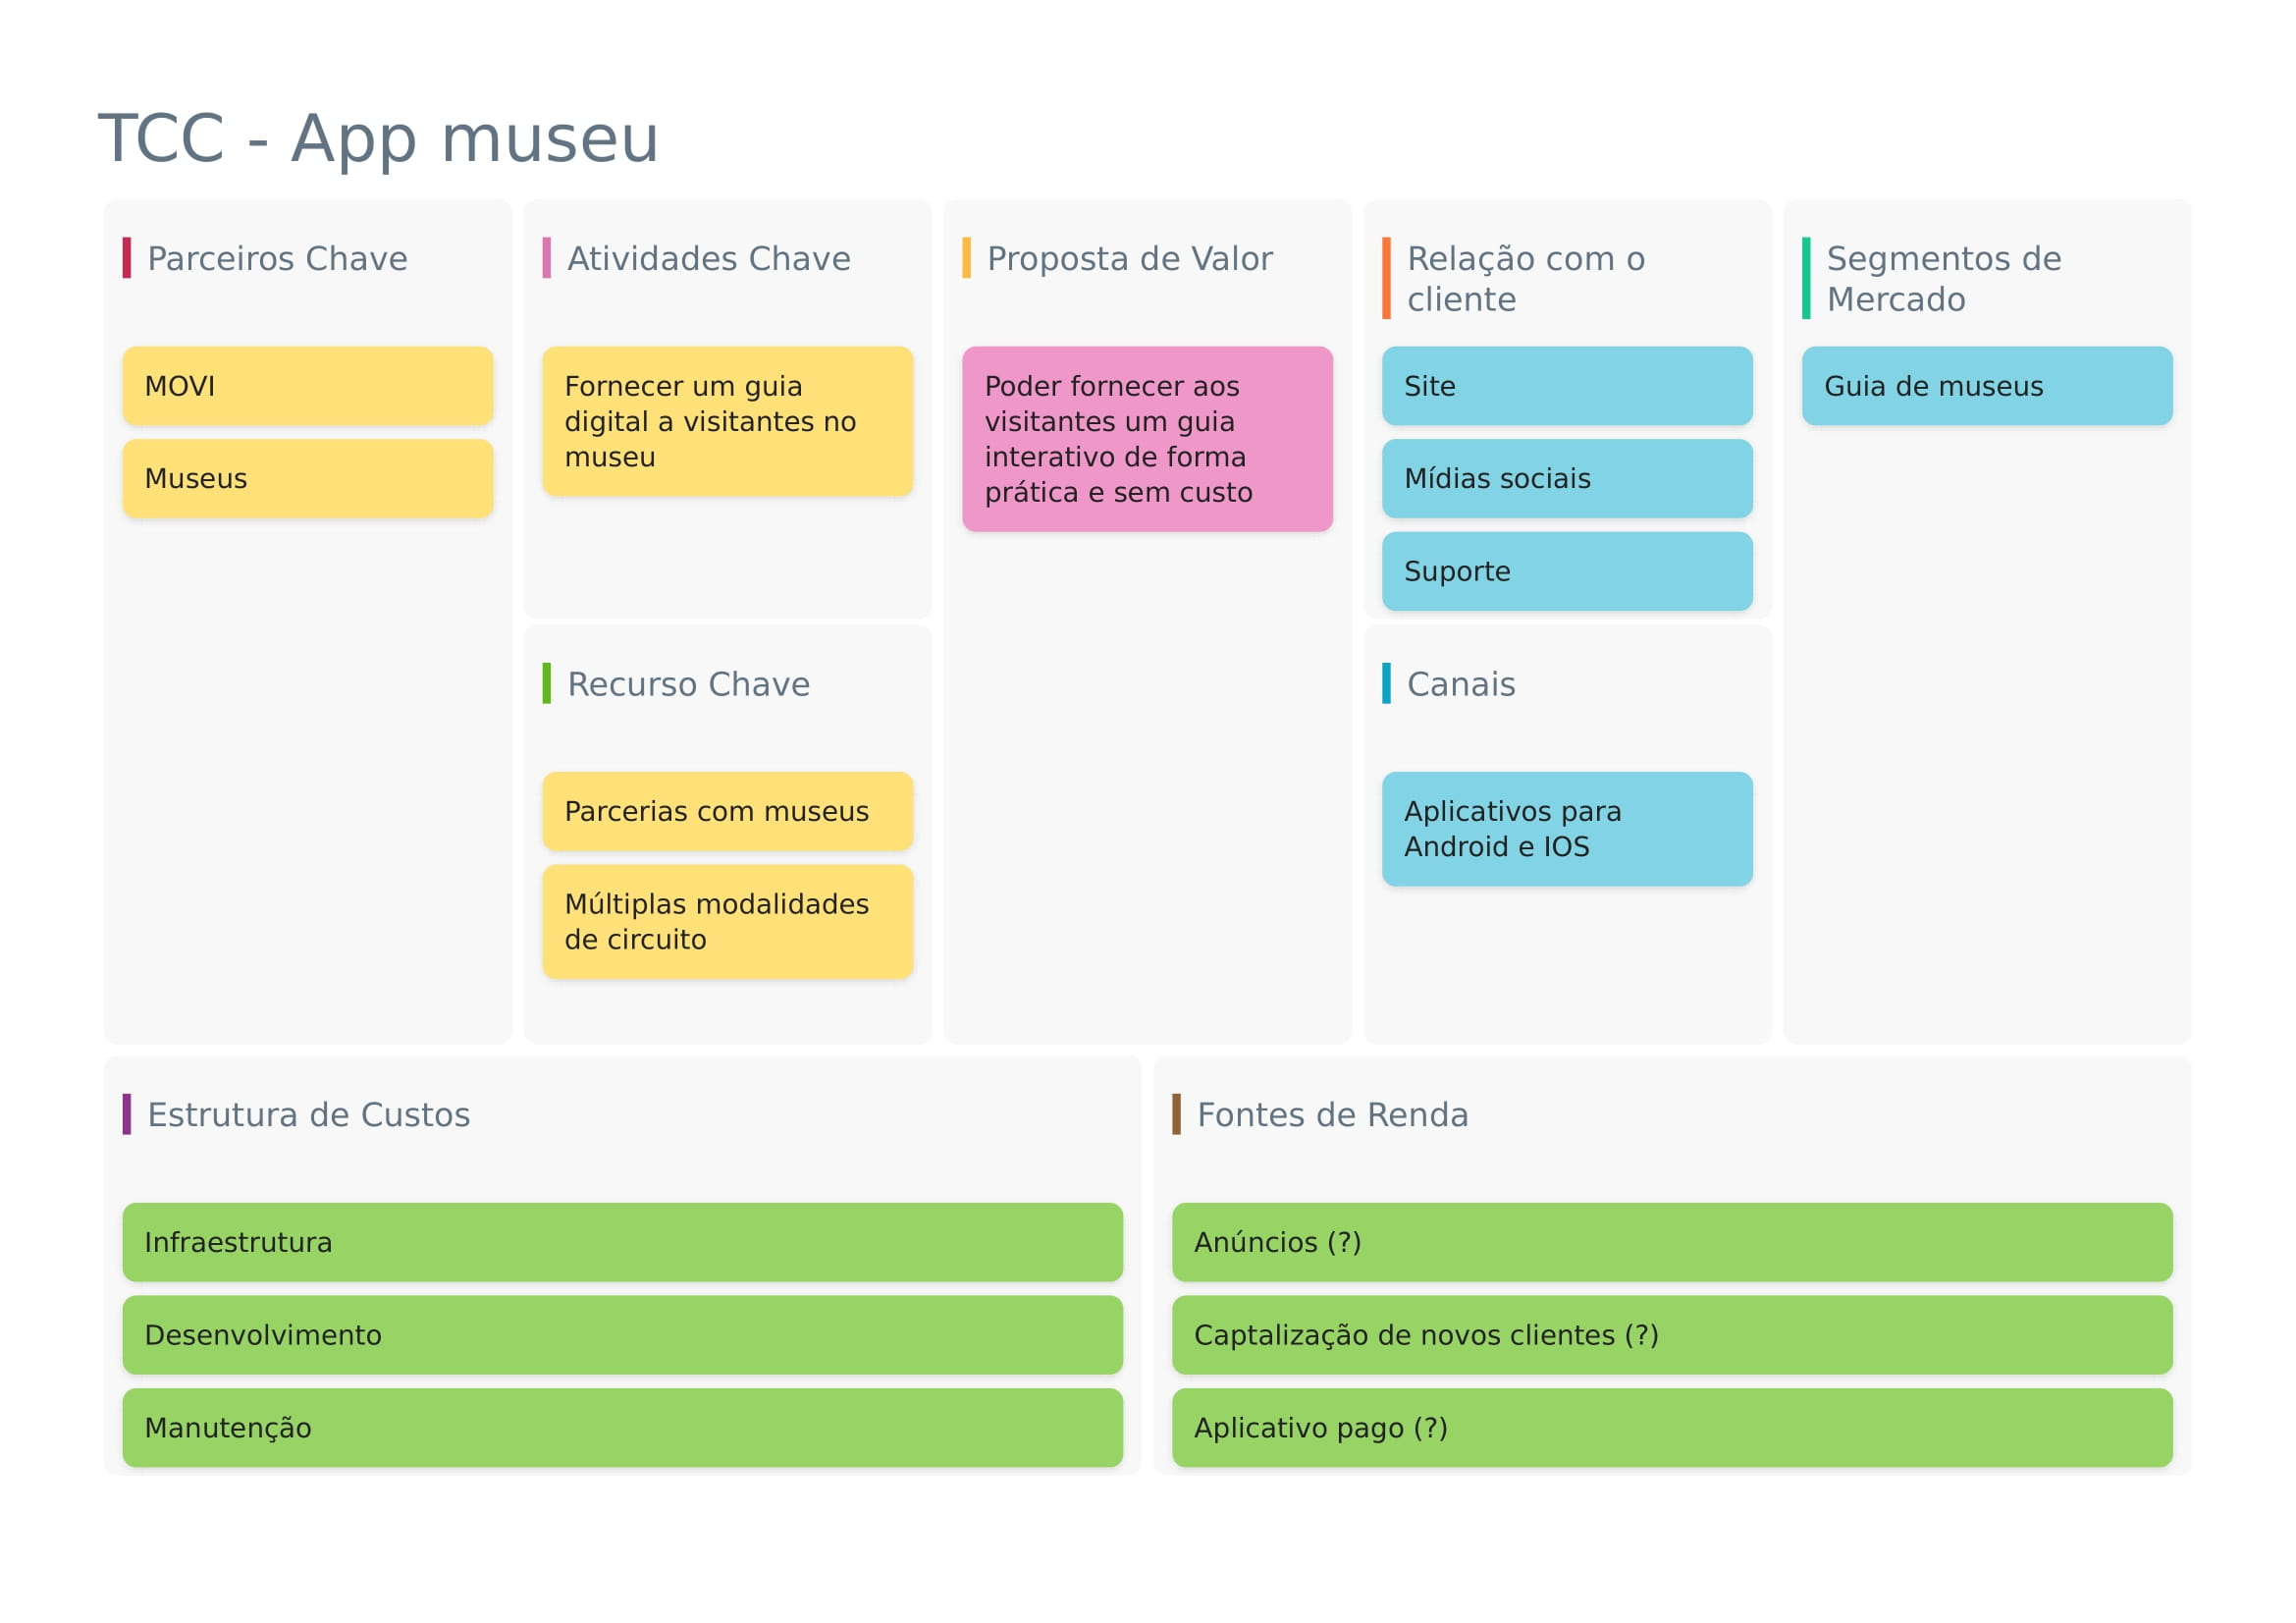
\includegraphics[width=0.975\textwidth]{images/canvas.jpg}
    }}
    \caption{AppNome Business Model Canvas}
    % \caption*{Fonte: Autor, 2022}
    \vspace{-0.3cm}
    \label{fig:canvas}
\end{figure}

Com a opção de um guia digital capaz de fornecer explicações sobre as obras, bem como poder encaminhar pessoas com deficiências para as mesmas, tornaria o museu mais acessível para todos.

\subsection{Delimitação do Escopo}

Este trabalho propõe-se a oferecer um aplicativo guia digital e um sistema de comunicação sem fio para que o MOVI seja capaz de interagir com PCDs visuais, e ter uma experiência mais amigável com seu público geral através do app. Contará com um sistema web de administradores para o cadastro de pontos de sensoriamento para ativação no guia, bem como cadastro de falas, e quizzes.

O quadro \ref{tab:VersioningVisitors} apresenta a tabela de versionamento do aplicativo para visitantes. Pretende-se neste trabalho implementar no mínimo o MVP \footnote{O MVP é aquela versão do produto que permite uma volta completa do ciclo construir-medir-aprender, com o mínimo de esforço e o menor tempo de desenvolvimento \cite{TheLeanStartup}} (Minimum Viable Product).

\renewcommand{\arraystretch}{1}
\begin{quadro}[H]
    \centering
    \caption{Versionamento do aplicativo para visitantes}
    \begin{tabular}{|m{0.75\textwidth}|m{0.16\textwidth}|}
        \hline
        \rowcolor[HTML]{C0C0C0}
        \textbf{Item} & \textbf{Versão} \\
        \hline
        Modalidade para público geral & MVP parcial \\
        \hline
        Cadastro de usuário & MVP parcial \\
        \hline
        Avaliação de conhecimentos (Quiz) & MVP final \\
        \hline
        Modalidade para PCDs visuais & MVP final \\
        \hline
        Suporte dentro do aplicativo & 1.1.0 \\
        \hline
        Avaliação do museu & 1.2.0 \\
        \hline
        Emblemas de usuário & 1.3.0 \\
        \hline
    \end{tabular}
    \vspace{-0.6cm}
    \label{tab:VersioningVisitors}
\end{quadro}
\renewcommand{\arraystretch}{1.1}

O quadro \ref{tab:VersioningAdmin} apresenta a tabela de versionamento do sistema web para administradores.

\renewcommand{\arraystretch}{1}
\begin{quadro}[H]
    \centering
    \caption{Versionamento do sistema web para administradores}
    \begin{tabular}{|m{0.75\textwidth}|m{0.16\textwidth}|}
        \hline
        \rowcolor[HTML]{C0C0C0}
        \textbf{Item} & \textbf{Versão} \\
        \hline
        Cadastro de novos administradores & MVP parcial \\
        \hline
        Cadastro de novos pontos & MVP final \\
        \hline
        Cadastro de novas falas & MVP final \\
        \hline
        Visualização de métricas & 1.1.0 \\
        \hline
    \end{tabular}
    \vspace{-0.6cm}
    \label{tab:VersioningAdmin}
\end{quadro}
\renewcommand{\arraystretch}{1.1}

Para a realização da comunicação do aplicativo com o museu, será integrado um sistema de comunicação sem fio às obras (ainda não foi estudado), que será capaz de fornecer ao guia digital as informações necessárias para ativação de falas, e a realização de quizzes.

\subsection{Justificativa}

Atualmente alguns museus possuem certas soluções alternativas além da visual para o auxílio de PCDs ou público geral, como o exemplo de áudio guias, ou QR codes para leitura de informações. No entanto, essas soluções existentes não contemplam todas as necessidades de um portador de deficiência visual (Falta colocar uma referência aqui, não achei o link dnv), nem facilitam completamente a visita do público geral, como a necessidade de se utilizar de aparelhos de terceiros \cite{Nintendo:Louvre}.

Com isso, pode-se observar a necessidade de encontrar uma solução que satisfaça as necessidades de um portador de deficiência visual, e que possa ser utilizada por todos os visitantes de forma mais facilitada e amigável. 

A ideia deste trabalho é oferecer uma solução que contemple os problemas abordados na seção 1.1 das soluções já existentes no mercado, na qual se assemelham ao aplicativo, porém com o diferencial de se utilizar o próprio celular do visitante, que seja capaz de fornecer uma experiência próxima de um guia real, sem a necessidade de pagar por um guia para o mesmo.

\section{LEVANTAMENTO DE APLICATIVOS EXISTENTES NO MERCADO}

Texto sobre o Levantamento de Aplicativos Existentes no Mercado

\subsection{Aplicativo X}

Resumo sobre o App X

\subsection{Aplicativo Y}

Resumo sobre o App X

\subsection{Comparativo de Funcionalidades}

Texto sobre a tabela.
Tabela de comparativo entre os Apps.

\section{OBJETIVOS}

\subsection{Objetivo Geral}

Desenvolver um guia digital mobile integrado com um sistema de comunicação
sem fio para oferecer uma experiência mais acessível a PcDs visuais e mais interativa ao visitante

\subsection{Objetivos Específicos}

\vspace*{0pt}

\begin{itemize}
	\item Comparar as principais técnicas de comunicação;
	
	\item Implementar dispositivos de sensoriamento nas obras para ativação do guia;

    \item Efetuar o levantamento de requisitos e modelagem do aplicativo;

    \item Desenvolver o aplicativo como guia digital com interação ao sistema de comunicação implantado; e
    
    \item Criar quizzes com gamificação.
    
\end{itemize}

\section{ESTRUTURA DO TRABALHO}

Texto sobre a estrutura aqui.
 \clearpage
\chapter{ESPECIFICAÇÃO DO PRODUTO}
\label{cap:espProd}
Neste capítulo, são as apresentadas as (i) as tecnologias escolhidas no desenvolvimento deste projeto e (ii) as documentações acerca das mesmas, como levantamento de requisitos, casos de uso e diagramas de sequência, tanto do aplicativo como do sistema web.

\section{MVP}

Texto sobre o MVP

\subsection{Tecnologias}

Texto sobre tecnologias

\subsubsection{Linguagem de programação Front-End}

Texto sobre o Front-End

\subsubsection{Linguagem de programação Back-End}

Texto sobre o Back-End

\subsubsection{Sistema de gerenciamento de banco de dados SQL}

Texto sobre o banco SQL

\subsubsection{Tecnologias de implantação}

Texto sobre a implementação das tecnologias.

\subsubsection{Tecnologias de hardware}

Texto sobre a implementação do hardware.

\section{DOCUMENTAÇÃO DO APLICATIVO}

% Nos itens a seguir serão demonstrados os requisitos do sistema, casos Nos itens a seguir serão demonstrados os requisitos do sistema, casos de uso, diagramas e protótipos. Eles serão divididos em quatro partes: (i) documentação do aplicativo móvel para clientes; (ii) documentação do aplicativo móvel para entregadores; (iii) diagrama de classes do back-end dos aplicativos; e (iv) diagrama de sequência das aplicações.

\subsection{Aplicativo para visitantes}

Texto sobre o aplicativo dos visitantes

\subsubsection{Especificação dos requisitos}
\subsubsection{Diagrama de casos de uso}
\subsubsection{Expansão de casos de uso}
\subsubsection{Diagrama de sequência}

\subsection{Sistema web para administradores}

Texto sobre o aplicativo dos visitantes

\subsubsection{Especificação dos requisitos}
\subsubsection{Diagrama de casos de uso}
\subsubsection{Expansão de casos de uso}
\subsubsection{Diagrama de sequência}

Texto sobre o sistema web dos administradores.

\subsection{Back-end da aplicação}

Texto sobre o o back-end da aplicação. \clearpage
\chapter{DESENVOLVIMENTO PARCIAL}
\label{cap:devParc}

Texto sobre o desenvolvimento parcial

\section{BACK-END}
\label{sec:premissas}

Texto sobre o back-end

\section{APLICATIVO E SISTEMA WEB}

Nesta subseção será demonstrado o processo de desenvolvimento do aplicativo para visitantes e o sistema web para administradores.

\subsection{Aplicativo para o público}

Texto sobre o back-end do aplicativo. + A interface do aplicativo de visitantes será dada a partir da prototipação de um TIC (Trabalho de iniciação cientifica), realizado pela acadêmica Louis de Design Gráfico.

\subsection{Sistema web para administradores}

Texto sobre o back-end do sistema web. \clearpage
\chapter{RESULTADOS PARCIAIS}
\label{cap:resultParc}

Nesta seção será descrito os métodos utilizados para a realização de testes de usabilidade para PCDs visuais acerca do aplicativo e do sistema web para administradores, bem como os resultados obtidos.

\section{TESTE DE COMUNICAÇÃO SEM FIO}

Texto de Teste da comunicação do aplicativo com o sistema de comunicação sem fio implantado.

\section{TESTE DE ACESSIBILIDADE PARA PCDs VISUAIS}

Texto de Teste de acessibilidade para PCDs visuais.

\section{TESTE DE USABILIDADE DE INTERFACE}

Texto sobre teste de usabilidade de interface.

\subsection{Teste de usabilidade do aplicativo}

Texto de usabilidade do aplicativo para o público geral e para PCDs.

\subsubsection{Observações}

Observações da descrição dos participantes.

Texto sobre o uso pelos participantes

\subsubsection{Questionário}

Texto sobre o questionário.
Imagens de resultados dos questionários.

\subsection{Teste de usabilidade da interface web}

Texto de teste de usabilidade interface web para administradores.

\subsubsection{Observações}

Observações da descrição dos participantes.

Texto sobre o uso pelos participantes

\subsubsection{Questionário}

Texto sobre o questionário.
Imagens de resultados dos questionários.
 \clearpage
\chapter{PLANEJAMENTO PARA O TCC III}
\label{cap:planTcc}

Texto de planejamento para o TCC III.

\section{Cronograma}

Falar sobre o quadro de cronograma (abaixo).

\vspace{10pt}

\begin{cronograma}
    {Cronograma de execução para o TTC III}
    \label{tab:cronograma3}
    \uHeaderCronograma{01/2023}{02/2023}{03/2023}{04/2023}{05/2023}{06/2023}
    \uAtividade{3.a) Implementação da comunicação}{XXXX}{XXXX}{}{}{}{}
    \uAtividade{3.d) Integração do app com o museu} {}{XXXX}{XXXX}{XX\nX\nX}{}{}
    \uAtividade{3.e) Desenvolver o roteiro de teste} {}{}{XXXX}{XXXX}{}{}
    \uAtividade{4.a) Verificação} {}{}{}{XXXX}{XXXX}{}
    \uAtividade{4.b) Testes} {}{}{}{XXXX}{XXXX}{}
    \uAtividade{5.a) Escrita do relatório do TTC }{XXXX}{XXXX}{XXXX}{XXXX}{XXXX}{XX\nX\nX}
\end{cronograma}

\section{Metodologia}

Texto sobre a metodologia

\section{Análise de riscos}

Texto sobre a análise de riscos.
 \clearpage
\chapter{ANÁLISE CRITICA}
\label{cap:anaCri}

Texto sobre análise critica
 \clearpage

\postextual

\bibliography{refs}

\end{document}
